% LaTeX source for ``การเรียนรู้ของเครื่องสำหรับเคมีควอนตัม (Machine Learning for Quantum Chemistry)''
% Copyright (c) 2022 รังสิมันต์ เกษแก้ว (Rangsiman Ketkaew).

% License: Creative Commons Attribution-NonCommercial-NoDerivatives 4.0 International (CC BY-NC-ND 4.0)
% https://creativecommons.org/licenses/by-nc-nd/4.0/

\chapter{การทำนายคุณสมบัติเชิงโมเลกุล}
\label{ch:predict_molprop}

%--------------------------
\section{Best Practice}
%--------------------------

Best Practice หรือแนวทางปฏิบัติหรือลำดับขั้นตอนสำหรับการนำ ML มาประยุกต์กับเคมีควอนตัมสามารถแบ่งออกเป็น 5 ขั้นตอนง่าย ๆ ได้ดังนี้
\idxen{Best Practice}

\begin{enumerate}
    \item การเลือก dataset
    \item การทำความสะอาดข้อมูลดิบ (raw data)
    \item คำนวณหา Representation ต่อไปได้ ซึ่งขั้นตอนนี้ก็สำคัญมาก ๆ เพราะการเลือก Representation 
    ที่จะใช้ในการเทรนโมเดลก็ต้องสอดคล้องกับ output ที่เราต้องการจะทำนาย -> และหลังจากนั้นก็เป็นขั้นตอนของ
    \item การเลือก ML algorithm เพื่อให้เหมาะสมกับโจทย์ของเรา 
    \item การเทรนโมเดลและการประเมินโมเดลโดยการทำ Validation
\end{enumerate}

\begin{figure}[H]
    \centering
    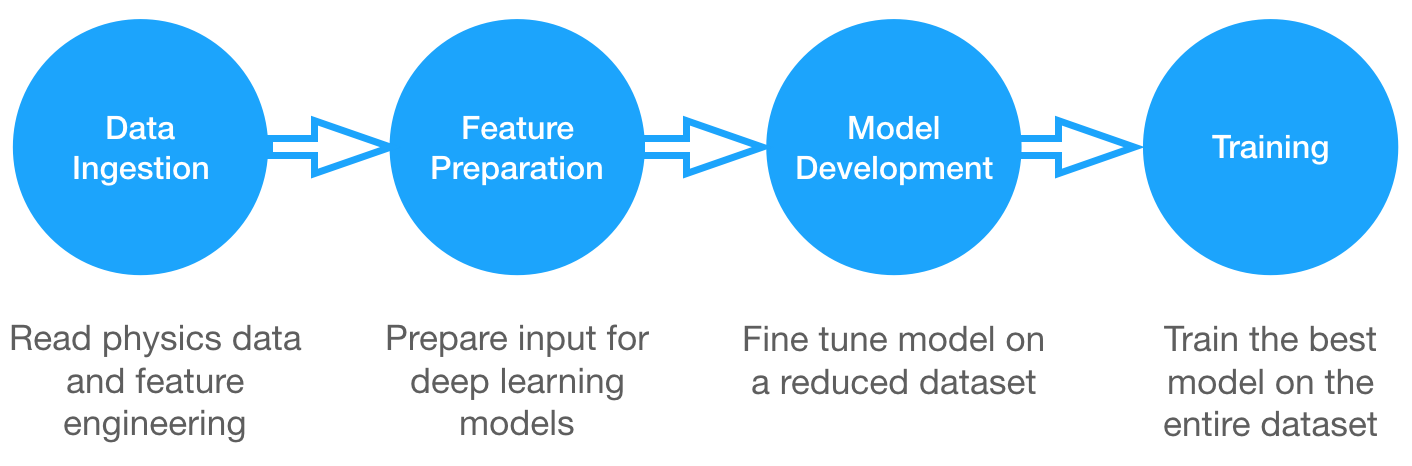
\includegraphics[width=0.9\linewidth]{fig/ml_pipeline.png}
    \caption{แนวทางและขั้นตอนการสร้างโมเดลปัญญาประดิษฐ์ (เครดิตภาพ: https://vitalflux.com)}
    \label{fig:ml_pipeline}
\end{figure}

%--------------------------
\section{การเลือกโมเดลที่เหมาะสม}
%--------------------------

\begin{figure}[H]
    \centering
    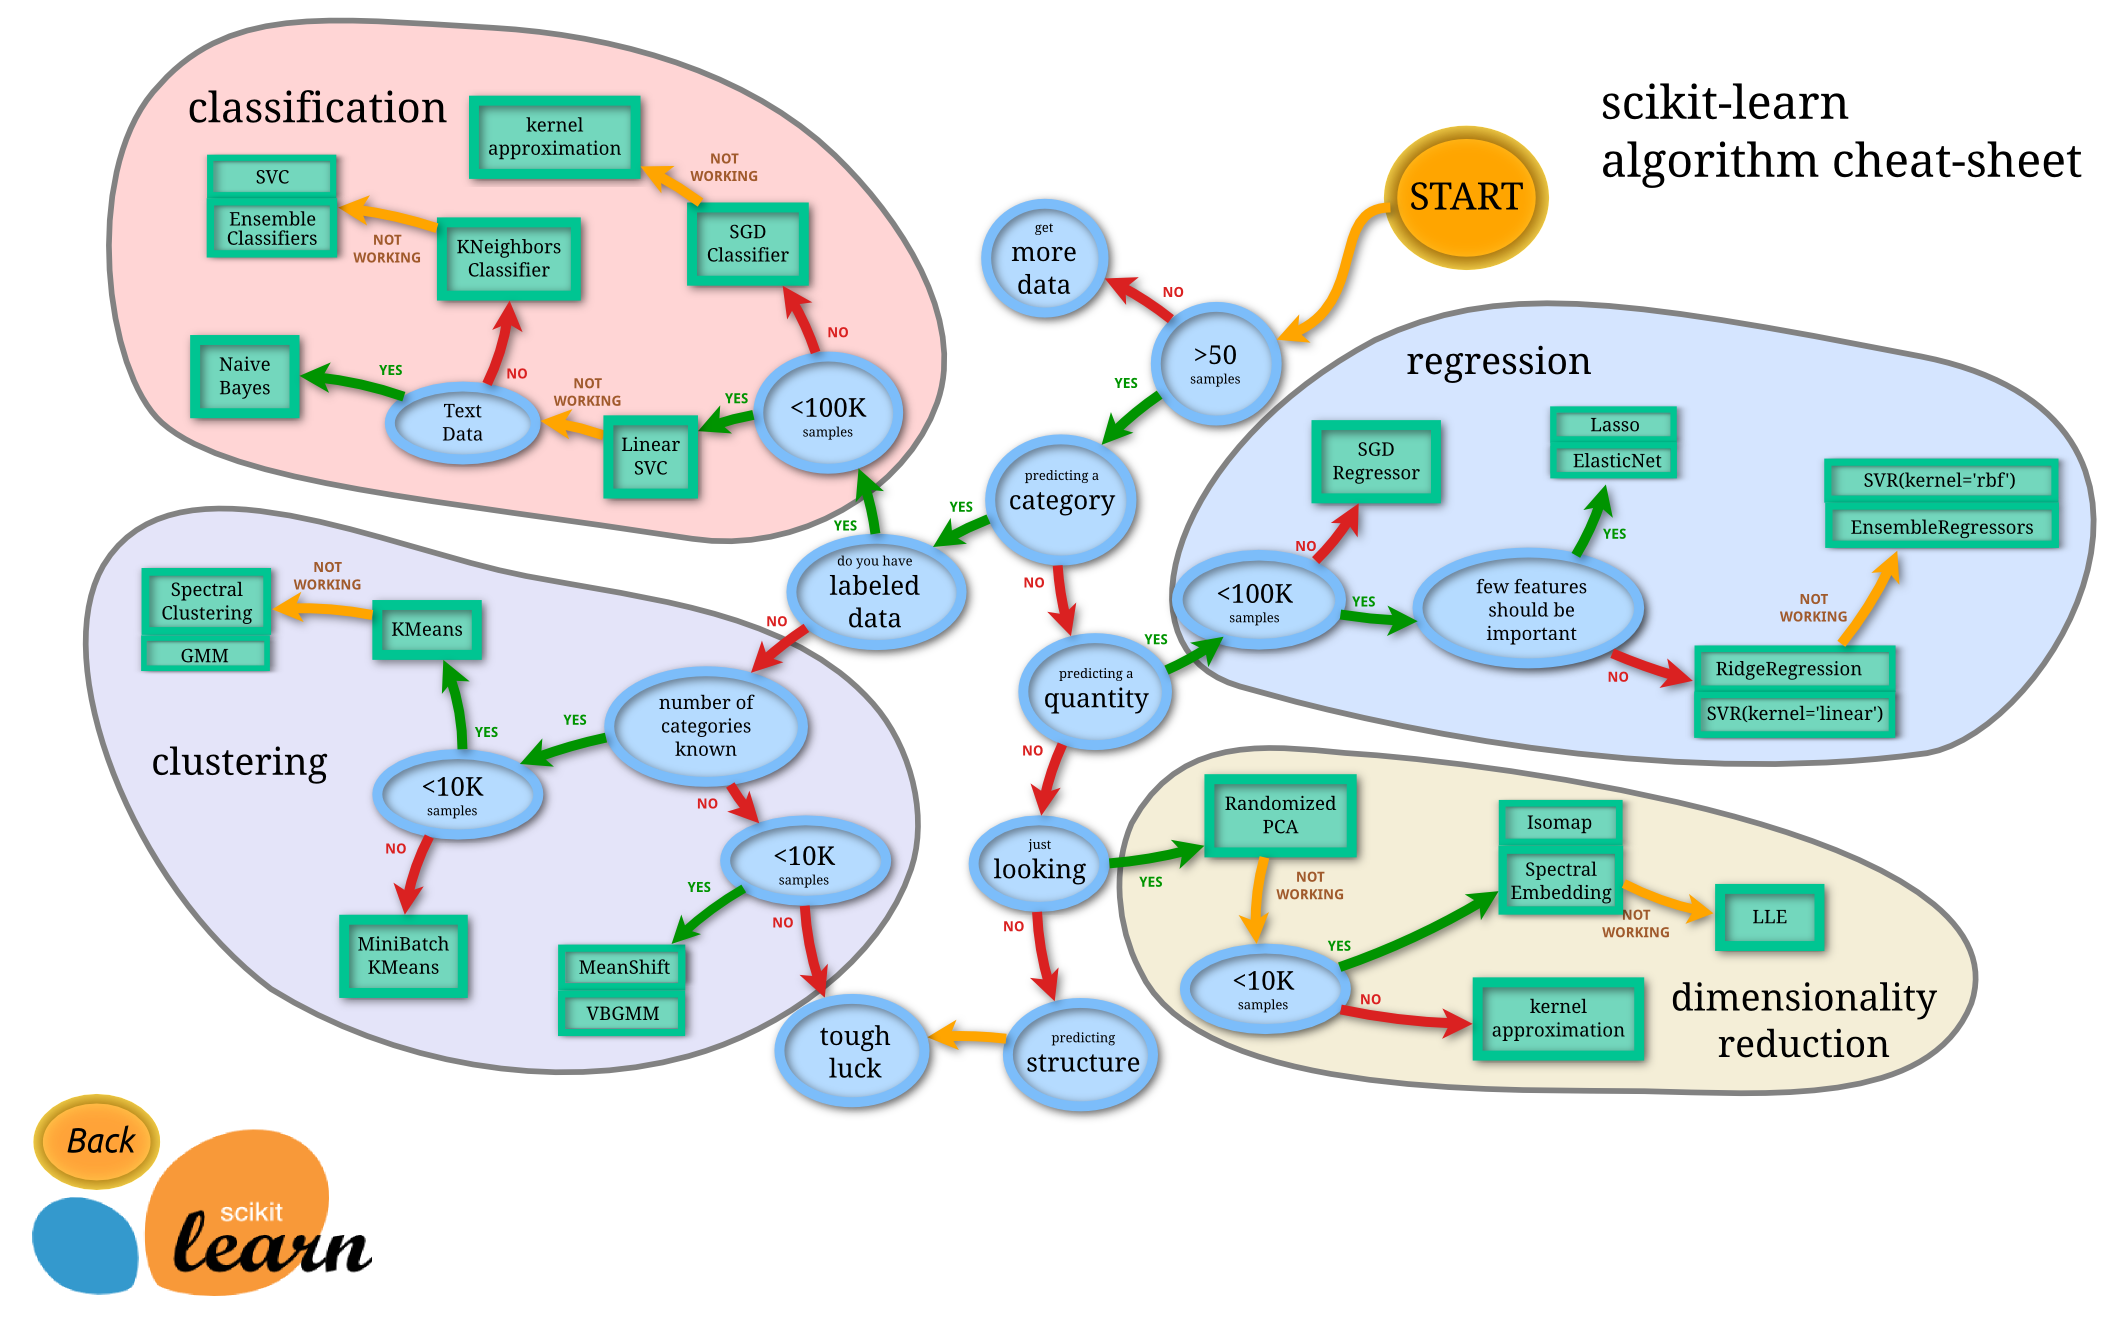
\includegraphics[width=0.9\linewidth]{fig/ml_map.png}
    \caption{แผนภาพการเลือกใช้โมเดลปัญญาประดิษฐ์ (เครดิตภาพ: https://scikit-learn.org)}
    \label{fig:ml_map}
\end{figure}

\begin{itemize}
    \item Linear kernel : $K(x_i, x_j) = x_i \cdot x_j$
    \item Polynomial : $K(x_i, x_j; a, b) = (x_i \cdot x_j + a)^b$
    \item Gaussian kernel : $K(x_i, x_j; w, \sigma) = \mathrm{exp}\left(-\frac{|x_i-x_j|^2}{2\sigma^2}\right)$
    \item Laplacian kernel : $K(x_i, x_j; w, \gamma) = \mathrm{exp}\left(-{|x_i-x_j|}\right)$
\end{itemize}

%--------------------------
\section{การทำนายพลังงาน Potential Energy Surface}
%--------------------------

การทำนายพื้นผิวพลังงานศักย์ (Potential Energy Surface หรือ PES)

Machine Learning Potentials (MLP) แบ่งออกได้เป็นสองประเภทคือ Kernel-based Potential กับ Neural Network-based Potential

- Gaussian Approximation Potentials (GAP)\cite{bartok2010}
- Moment Tensor Potentials (MTP)\cite{shapeev2016}
- Spectral Neighbor Analysis Potentials (SNAP)\cite{thompson2015}


- High-dimensional Neural Network Potentials (HDNNP)\cite{behler2007}
- ANAKIN-ME หรือเรียกสั้น ๆ ว่า ANI (ชื่อเต็มคือ (Accurate NeurAl networK engINe for Molecular Energies)
    - ANI-1x\cite{smith2017}
    - ANI-1ccx\cite{smith2018}
    - ANI-2x\cite{smith2019}

%--------------------------
\section{การจำลอง Force Field}
%--------------------------

การทำนายหรือพยากรณ์แรง (Forces) และพลังงาน (Energies) ของโมเลกุลนั้นเรียกอีกอย่างหนึ่งว่าการสร้างโมเดล ML Force-field 
เริ่มต้นสมมติว่าเรามีชุดข้อมูลที่มี Feature Vector ซึ่งเขียนแทนด้วย $\mathbf{D}$ และมีอนุพันธ์แบบเวกเตอร์ (Divergence) เป็น 
$\nabla_{\mathbf{r_i}} \mathbf{D}$ และมีข้อมูลเพิ่มเติมคือพลังงาน $E$ และแรง $\mathbf{F}$ ของระบบ (โมเลกุล) สำหรับการฝึกสอน
เราจะสร้าง Neural Network (เขียนแทนด้วย $f$) เพื่อสร้างโมเดลสำหรับการทำนายพลังงาน ($\hat{E} = f(\mathbf{D})$)
\footnote{ตัวแปรที่มีเครื่องหมาย $\hat{}$\,(อ่านว่า \enquote{hat}) อยู่ด้านบนจะบ่งบอกถึงค่าที่เราจะทำนายของตัวแปรหรือมาณนั้น ๆ}
ซึ่งเราสามารถคำนวณแรงได้โดยตรงจากค่าติดลบของ Gradient ของพลังงานเทียบกับพิกัดตำแหน่งของอะตอมนั้น ๆ ดังนั้นแรงที่ได้จะเป็นปริมาณต่ออะตอม
ยกตัวอย่างเช่นแรงของอะตอม $i$ สามารถคำนวณได้จากสมการต่อไปนี้ (โดยใช้เวกเตอร์แบบแถว)
\idxen{Force Field}

\begin{align}\label{eq:force_pred}
\hat{\mathbf{F}}_i &= - \nabla_{\mathbf{r_i}} f(\mathbf{D}) \\
&= - \nabla_{\mathbf{D}} f \cdot \nabla_{\mathbf{r_i}} \mathbf{D}\\
&= - \begin{bmatrix}
    \frac{\partial f}{\partial D_1} & \frac{\partial f}{\partial D_2} & \dots
\end{bmatrix}
\begin{bmatrix}
    \frac{\partial D_1}{\partial x_i} & \frac{\partial D_1}{\partial y_i} & \frac{\partial D_1}{\partial z_i}\\
    \frac{\partial D_2}{\partial x_i} & \frac{\partial D_2}{\partial y_i} & \frac{\partial D_2}{\partial z_i}\\
    \vdots & \vdots & \vdots \\
\end{bmatrix}
\end{align}

จากสมการ \ref{eq:force_pred} นั้นเราอธิบายได้ว่า $\nabla_{\mathbf{D}} f$ เป็นค่าอนุพันธ์ของคำตอบของโมเดล ML ซึ่งจะเทียบกับ%
Descriptor $\mathbf{D}$ และ $\nabla_{\mathbf{r_i}} \mathbf{D}$ เป็น อนุพันธ์ของ Descriptor ที่เทียบกับตำแหน่งของอะตอม
ซึ่งตามที่เราได้ศึกษามาก่อนหน้านี้ว่า Neural Network นั้นจะให้คำตอบที่เป็นแบบ Analytical Solution

%--------------------------
\section{การทำนายพลังงานกระตุ้นของปฏิกิริยาเคมี}
%--------------------------

Activation energy หรือพลังงานกระตุ้น เป็นค่าพลังงานที่บ่งบอกถึงความยากง่ายในการทำให้ปฏิริยาเคมีสามารถดำเนินไปได้ ณ สภาวะหนึ่ง ๆ

%--------------------------
\section{การทำนาย Dipole Moment}
%--------------------------

%--------------------------
\section{การทำนาย Electronic Coupling}
%--------------------------

Electronic Coupling คือค่าความเกี่ยวเนื่องเชิงอิเล็กทรอนิกส์ระหว่าง 2 สถานะใด ๆ เช่นสถานะเริ่มต้นและสถานะสิ้นสุดในกระบวนการทางควอนตัม

- Nonadiabatic Coupling
- Electron transfer Coupling

%--------------------------
\section{การทำนายสเปคตรัม}
%--------------------------


%--------------------------
\section{บทความวิชาการเพิ่มเติม}
%--------------------------

นอกเหนือจากการนำ ML ไปใช้สำหรับการทำนาย Parameter ต่าง ๆ แล้ว ถ้าหากผู้อ่านสนใจการประยุกต์ใช้ ML กับงานทางด้านอื่น ๆ ของเคมีควอนตัม 
สามารถอ่านบทความวิชาการเพิ่มเติมได้จากวารสารวิชาการชั้นแนวหน้า เช่น Journal of Chemical Theory and Computation (JCTC), 
Journal of Chemical Physics (JCP), และ Journal of Physical Chemistry A (JPCA)

โดยผู้เขียนได้เลือกงานวิจัยที่มีความโดดเด่นและเหมาะสำหรับผู้เริ่มต้นศึกษาเป็นอย่างยิ่ง ซึ่งน่าจะช่วยให้ผู้อ่านเห็นภาพรวมของโจทย์งานวิจัยในปัจจุบันที่กำลังมาแรง
บทความที่คัดเลือกมาประกอบไปด้วย Review ที่ใช้ ML ในการเรียนรู้ Force Field สำหรับงานทางด้าน QM/MD หรือนำมาใช้ในการทำนาย Free Energy Landscape 
ไปจนถึงการพัฒนา Model ML เพื่อทำนาย Molecular Properties เช่น Dipole Moment และ Polarizability 

\begin{enumerate}
    \item \enquote{PhysNet: A Neural Network for Predicting Energies, Forces, Dipole Moments, and Partial Charges}\cite{unke2019}\\
    ตีพิมพ์เมื่อวันที่ 01 พฤษภาคม ค.ศ. 2019
    
    \item \enquote{Comparison of the Performance of Machine Learning Models in Representing High-Dimensional Free Energy Surfaces and Generating Observables}\cite{cendagorta2020}\\
    ตีพิมพ์เมื่อวันที่ 10 เมษายน ค.ศ. 2020
    
    \item \enquote{Kernel-Based Machine Learning for Efficient Simulations of Molecular Liquids}\cite{scherer2020}\\
    ตีพิมพ์เมื่อวันที่ 13 เมษายน ค.ศ. 2020

    \item \enquote{Machine Learning Force Fields}\cite{unke2021}\\
    ตีพิมพ์เมื่อวันที่ 11 มีนาคม ค.ศ. 2021\\

    \item \enquote{The Rise of Neural Networks for Materials and Chemical Dynamics}\cite{kulichenko2021}\\
    ตีพิมพ์เมื่อวันที่ 1 กรกฎาคม ค.ศ. 2021\\

\end{enumerate}
